\graphicspath{{chapters/07/images/}}
\chapter{Reali}


\section{Introduction}

The course follows the structure of the article
\textbf{\emph{Optimization Algorithms for Computational Systems
Biology.}}


\subsection{Definition of a system}

A system is a set of integrated and interacting \emph{components} or
\emph{entities} that form a whole with definite boundaries and
surrounding environment. A system has a goal to achieve by performing
one or more functions or tasks. Systems can be aggregated into a
\textbf{\emph{hierarchy}}. A system at a given level of detail can be a
component at a higher level of detail.

\begin{itemize}
\tightlist
\item
  A \textbf{\emph{complex}} (non-linear) \textbf{\emph{system}} is a
  system that does not satisfy the principle of superposition, i.e., the
  behavior of the system cannot be inferred from the behavior of its
  components.
\item
  A \textbf{\emph{dynamical system}} is a system where fixed rules
  define the time dependencies of the system in a geometrical space.
  Dynamical systems have a space and time dimension because they change
  their characteristics over time. If we pick snapshots of the system at
  different time points, we observe different configurations of the
  system (data).
\end{itemize}
\noindent
A \textbf{\emph{configuration}} or state of the system refers to the
current condition of the system and stores enough information to predict
its next move. A state is characterized by the position of its
components in a geometrical space and by the values of the attributes of
its components (e.g., concentration or number of each elements
involved). Systems change their state over time by changing the location
of some of their components or changing the attributes of some of their
components.

\begin{itemize}
\tightlist
\item
  \textbf{\emph{steady state}}: some of the attributes of the system are
  no longer changing in the future.
\item
  \textbf{\emph{transient state}}: time needed to reach the steady state.
\end{itemize}


\subsection{Determinism, nondeterminism, or stochasticity?}

\begin{itemize}
\tightlist
\item
  \textbf{\emph{Deterministic systems}} always react in the same way to
  the same set of stimuli. These systems are completely determined by
  the initial state and the input set. The essence of deterministic
  systems is that each event is causally related to previous events and
  choices are always resolved in the same way in the same context. When
  a system generates multiple outcomes from the same input in different
  observations, the system is \textbf{\emph{nondeterministic}} (we
  cannot predict the output from the input).
\item
  \textbf{\emph{Stochasticity}} is the quality of lacking any
  predictable order or plan and stochastic systems possess some inherent
  randomness. It is possible to transform a nondeterministic system into
  a stochastic one by attaching probabilities to the selection points so
  that we turn nondeterministic choices into probabilistic choices.
\end{itemize}


\subsection{Computational complexity}

Complexity arises when interacting components self-organize to form
evolving structures that exhibit a hierarchy of emergent system
properties. An \textbf{\emph{emergent behavior}} can be originated by a
collection of components that interact in the absence of a centralized
point of control to produce something that has not been designed or
programmed in the system construction or evolution. Example: internet,
ant colonies, consciousness.\\
\\
\noindent
\textbf{\emph{Computational complexity}} is the amount of resources,
measured as a function of the size of the input, needed to execute an
algorithm.

\begin{itemize}
\tightlist
\item
  Computational space complexity: the amount of memory needed;
\item
  Computational time complexity: the number of instructions to be
  executed.
\end{itemize}


\subsection{Definition of a model}

A \emph{representation} is a set of symbols used to convey information
and knowledge about a system. It is either physical as a cell or an
ecosystem, or artificial as a computer network or an economic market. An
abstraction is a representation that ignores some aspects of a system
which are not of interest for the current investigation.
\\
\\
\noindent
A \emph{model} is an abstraction of a system. A model has its own interacting
components that are characterized by the attributes that we want to
observe. The set of all the attributes in a model is the
\emph{experimental frame}.

\begin{itemize}
\item
  A \emph{dynamic model} aims at predicting the behavior of the system
  in time/space through what if analysis. \textbf{What if analysis} investigates
  how a change in some attributes affects the behavior of the modeled
  system.
\item
  A \emph{computational model} is a model that can be manipulated by a
  computer to observe properties of the corresponding system.

  \begin{figure}
  \centering
  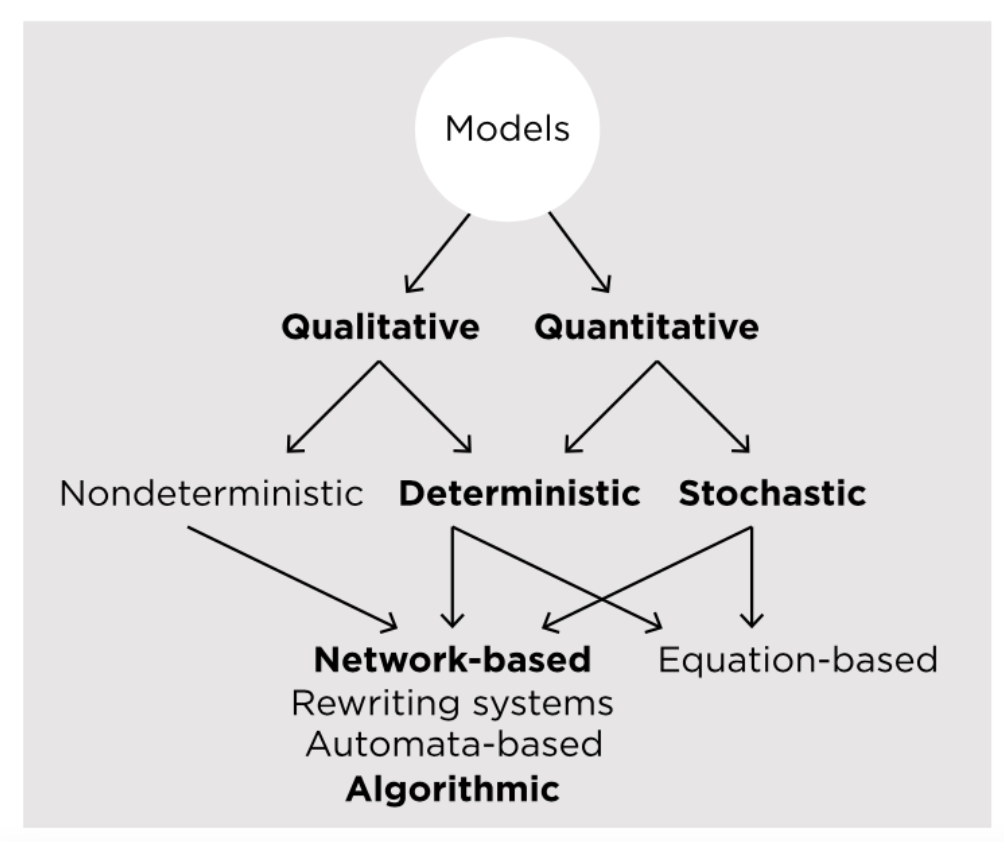
\includegraphics[width=0.6\textwidth]{scheme_model.png}
  \caption{From a model to methods}
  \end{figure}
\end{itemize}


\subsection{Checking the validity of a model}

\emph{Validity} is a fundamental property of models and witnesses the
capacity of a model of making good predictions. We need to assess the validity of a
model before using it to predict the behavior of a system.
\\
\\
\noindent
Assume that $M$ is a model for the system $S$ and $\underline{M}$ is the
modeling process. Let $s(t)$ and $m(t)$ be the state of the system and
of the model at time $t$, and $f_s$ and $f_m$ the state transition
functions of the system and of the model, respectively. Finally, let
$I_s(t)$ and $O_s(t)$ be the input and output of the system at time $t$.
Similarly, we write $I_m(t)$ and $O_m(t)$ for the model.
\\
\\
\noindent
What we expect is that going from one state to the other we have a
function (one for the system and one for the model); in a mathematical
model we integrate the $f_m$ function to known what happens in the
transition of the model, but we cannot do that in the real setting (the
transition function $f_s$ is not known) → when dealing with nature, we
cannot validate models according to the previous definition, so we use
I/O validity, based on known input and outputs of the system.
\\
\\
\noindent
The input and output are here generalized concepts: input can be any
perturbation of the system or of the model, and output can be any
observable property causally related to the input.
\\
\\
\noindent
A model $M$ is valid for a system $S$ if:
$f_m(\underline{M}(s(t_0))) = \underline{M}(f_s(s(t_0))) = m(t_1)$

\begin{figure}
\centering
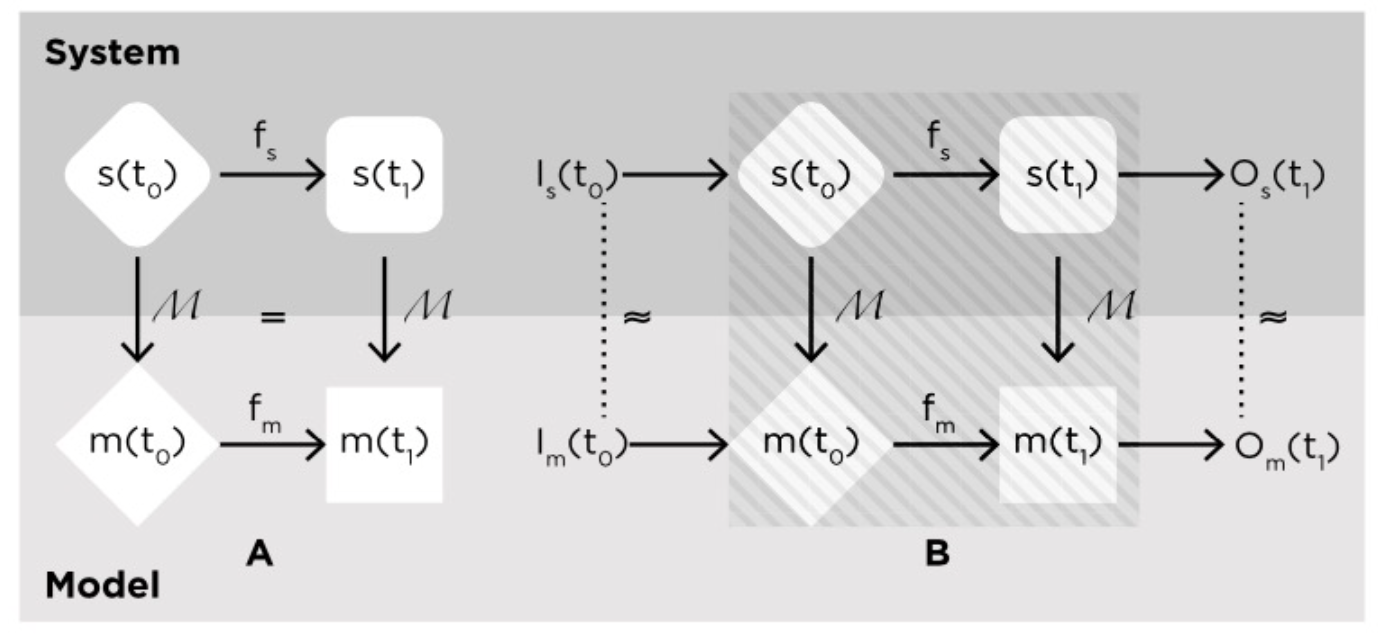
\includegraphics[width=0.7\textwidth]{validation.png}
\caption{validation}
\end{figure}
\noindent
I/O validity can be checked by using data sets produced by the model and
observed and measured on the system. An issue in this comparison process
is \emph{overfitting}:

\begin{itemize}
\tightlist
\item
  a model is well tuned to a specific dataset used to build the model
\item
  it performs poorly on other datasets
\end{itemize}
\noindent
\textbf{Cross-validation}: check overfitting by testing the model on
data sets different from the ones used to build and calibrate/train the
model.
\\
\\
\noindent
These concepts, even if usually referred to computational models, may
apply to general models or representations of a system.


\subsection{How to build a model}

We need to define objectives:

\begin{itemize}
\tightlist
\item
  what do you want to model?
\item
  what do you want to investigate with the model?
\item
  what do you expect from the model?
\item
  why do you need a model?
\end{itemize}

\begin{figure}
\centering
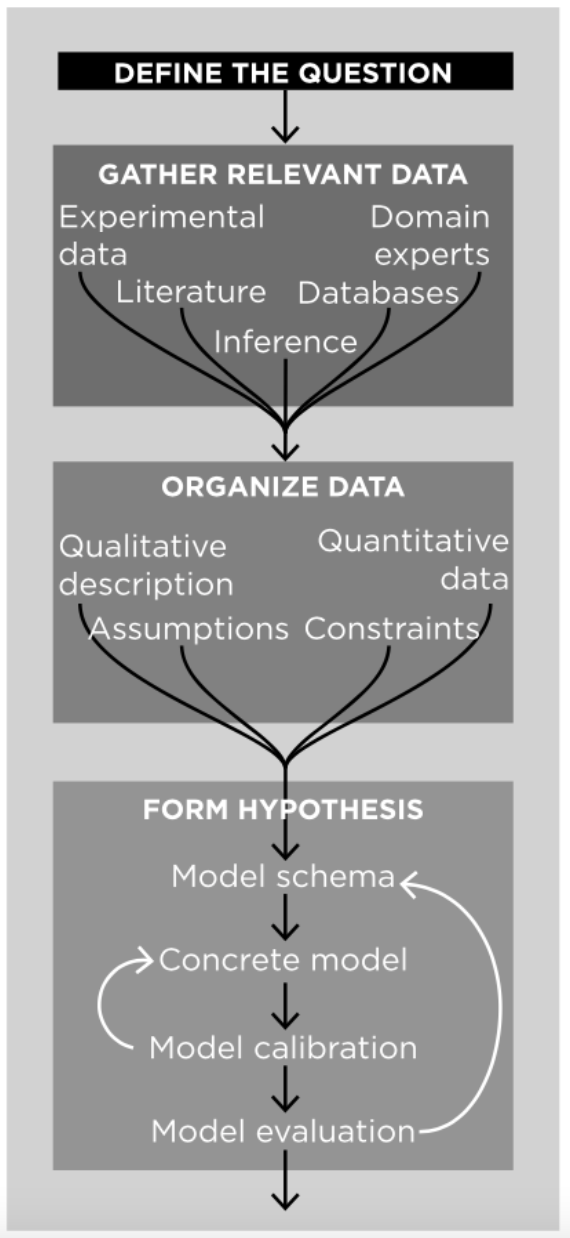
\includegraphics[width=0.3\textwidth]{workflow.png}
\caption{Workflow}
\end{figure}

\noindent
After defining the question and gathering data, we need to build the
model and calibrate it, in order to check if it can recapitulate data.
If it does not, either we are missing something or we must tune some
parameters. Different parameters can lead to dramatic changes in
dynamics. Example: Lotka-Volterra model with different parameter
conditions (Figure \ref{fig:Volterra}).

\begin{figure}
\centering
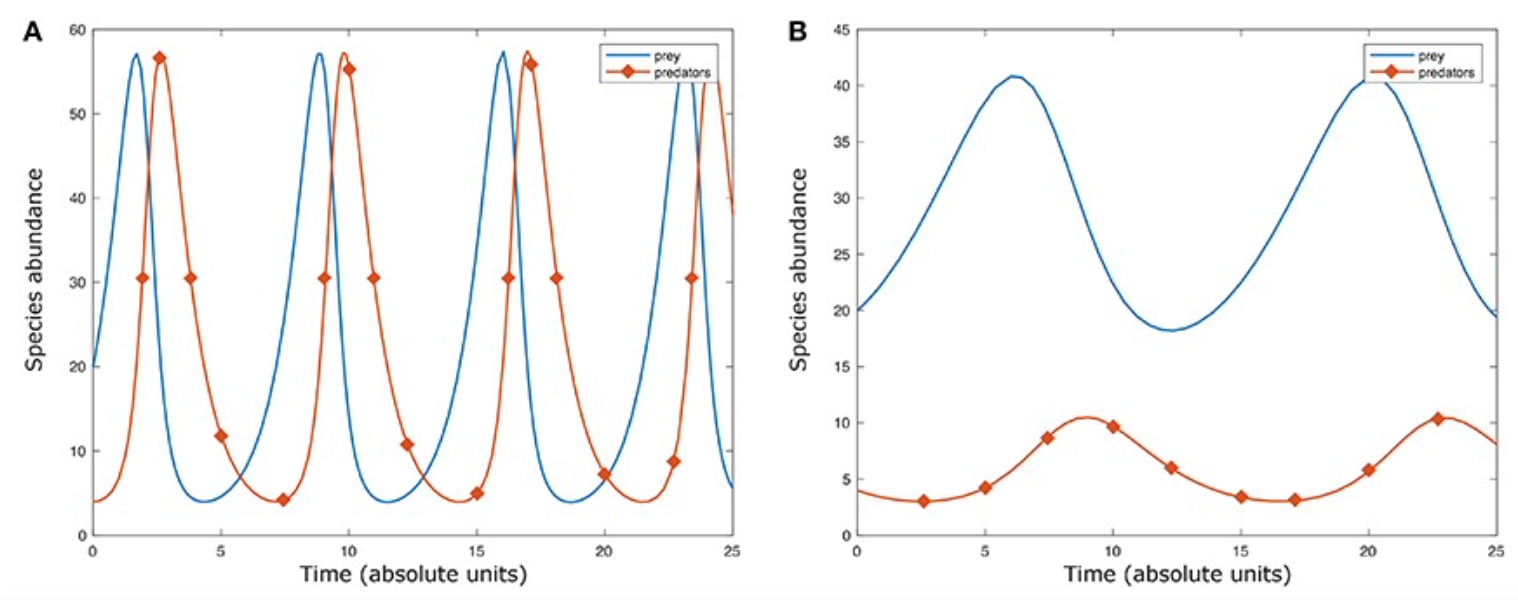
\includegraphics[width=\textwidth]{volterra.png}
\caption{Volterra}
\label{fig:Volterra}
\end{figure}

\begin{enumerate}
\def\labelenumi{\Alph{enumi})}
\item
  shows periodic oscillations, same amount of preys and predators
\item
  wider peaks and lower predator presence
\end{enumerate}

\section{Optimization problem}

In general, it is a problem in which we try to \emph{maximize} or \emph{minimize}
something. What we want to optimize is a function usually called
\emph{objective function} (or cost function). The function depends on a
variable or a vector of variables, called unknowns or parameters or
parameter estimates. They may be subject to certain
constraints(\textless,\textgreater,=).

\subsection{General definition of an optimization problem}

$\left.\left\{\begin{array}{ll} \max _{x \in \mathbb{R}^n} f(x) & \\ c_i(x)=0 & i=\mathcal{E}\\ f_j(x) \geq 0 & j = I \end{array}\right\} \text { set of indexes }\right] \text { Constraints (equality and inequality) }$
\\
\\
\noindent
The model (for us) is a function that gives a certain interval/time,
initial conditions and parameters, returns the variables at that time.
(Assume deterministic description)

$m: \mathbb{R} \times \mathbb{R}^{(n+1)} \times \mathbb{R}^m \rightarrow \mathbb{R}^N$

where n+1 accounts for the dimension of variables and time.

$$
\left(t_1,\left(\vec{x}_0, t_0\right), \theta\right)
\longmapsto \vec{x}_1 $$

Initial conditions in Lotka-Volterra: $((20,5), 0)$. 
\\
\\
\noindent
$\theta$ represents parameters e.g.~in Lotka-Volterra, $a,b,\beta,\alpha$. Now, assume that we have $k$ observations:

$(t_i ,\vec{y}_i), i=1, \ldots k$ , where
$t_i \in \mathbb{R}^+, \vec{y}_i \in \mathbb{R}^\ell$
\noindent
$y$ in theory can be a subset, $\ell<N$ : this happens a lot in complex
systems, we may not observe all variables! For simplicity, we can assume
$\ell=N$. Assuming that we can compute the following:

$$m\left(t_1,\left(\vec{x}_0, t_0\right), \theta\right) \in \mathbb{R}^{N} =_{\text{drop initial point notation}} m(t_i,\theta)$$
\noindent
We can compute distance: $d_i=\vec{y}_i-m(t_i, \theta)$.
\noindent
We can choose any type of distance (Euclidean, max\ldots). What we do is
calculating point-wise the distance between the model and `true' labels.
It is quite common to use the \textbf{\emph{Euclidean distance}}:
$$d \varepsilon =\sqrt{\sum_{i=1}^k(\vec{y}_i,-m(t_i, \theta))^2}\\
\rightarrow d{\varepsilon}-\sqrt{\sum_{i=1}^{K} \sum_{j=1}^{N} \left(y_{ij}-m_j\left(t_i, \theta\right)\right)^2}$$
\noindent
Sometimes we need need to add weights, which multiply each component in
the distances. We are putting together many outputs from the same model,
so we might want to scale everything to make it more comparable.
Furthermore, variables might be in different units of measurement,
leading to biased results.
\\
\\
\noindent
Observations:

\begin{itemize}
\tightlist
\item
  we do not want to reach ``zero'' when minimizing. Indeed, if the
  residual error $=0$, we are $100 \%$ sure that we are overfitting the
  data.
\item
  we need to really understand the data to construct the model
\item
  we are manipulating $\theta$ in the space of the parameters, but we
  modify the output in the space of the observations: we are connecting
  abstract values to observations - like parameters for maximum
  likelihood.
\end{itemize}

\noindent
Weights are multiplicative factors, sometimes we might wish to
\emph{transform} the distance. 
\\
\\
\noindent
Example:  \textbf{Least squares algorithm}

$$d{\varepsilon}=\sqrt{\sum \sum W_{ij}\left(y_{ij}-m_j\left(t_i, \theta\right)\right)}$$

\noindent
Our problem is to minimize/maximize a function. Assume:

$$
\min f(x), x \in \mathbb{R}^n
$$

\subsection{Definition of a minimum}

A point $x^*$ is called \textbf{minimum} if
$\exists \varepsilon > 0 : \forall x : || x- x^* || < \varepsilon$

$$
\Rightarrow f(x) \geq f(x^*) \\ 
$$
\noindent
{[}For the maximum $f(x) \leq f(x^*)${]}
\\
\\
\noindent
The minimum is \textbf{\emph{global}} if $\forall x \in \mathbb{R}^n$
(or in our domain) $f(x) \geq f(x^*)$. In general it is not easy to
determine global minimum/maximum, especially if we have a lot of
dimensions.
\noindent
To find minima or maxima, we should impose $f'(x)=0$.
\\
\\
\noindent
We call a \textbf{\emph{stationary point}}, a
$\bar{x} \text{ s.t.} f'(\bar{x})=0$.


\section{Gradient methods}

When we integrate to find ODE solutions, we do not obtain a function as
a solution, just points. In our optimization problem we do not know $f$ and $f'$(only sometimes
we do), so we are required to use \emph{numerical approximation}. The idea of
looking at $f'$ and set $f'=0$ is still at the base of gradient methods.
\\
\\
\noindent
If the problem contains constraints, how do we solve it? In this case
the problem is:

$$\left\{\begin{array}{ll}
\max f(x) &  \\
g_i(x)=0, & i \in \mathcal{I} \\
x \in \mathbb{R}^N
\end{array}\right.$$
\noindent
Let $\mathcal{I}= 1,...,m$. The traditional way to solve this problem is
to translate this system to another function. The Lagrangian function is
used to take into account the constraints.


\subsubsection{Lagrangian function}

We define the \textbf{\emph{Lagrangian function}} as
$L: \mathbb{R}^n \times \mathbb{R}^m \rightarrow \mathbb{R}$ s.t.

$$
L(x)= f(x) + \lambda g(x) = f(x) + \sum_{j=1}^m \lambda_j g_j(x)
$$


\subsection{Lagrangian Multipliers Theorem}

If $x^*$ is a stationary point for (Lagrangian function), then
$\exists \lambda^*$ s.t. $(x^* \lambda^*)$ is a stationary point for L. It
is a necessary condition (not sufficient, only one direction). This is a ``bigger'' problem, from
$\mathbb{R}^N \rightarrow \mathbb{R}^N \times \mathbb{R}^m$ . But still,
I can search solutions using stationary points. We can generalize the
idea to $g_i(x) \leq 0,$ constraints
\\
\\
\noindent
Remember that stationary points are not necessarily minima and maxima.
We check whether a stationary point is a max/min through second
derivations or evaluate the function in ``other'' points.

\subsection{Definition of a gradient}

Let $f: \mathbb{R}^N \rightarrow \mathbb{R}$ a differentiable function, we call gradient of $f$

$\nabla f: \mathbb{R}^N \rightarrow \mathbb{R}^N$ sit.
$\nabla f_i=\frac{\partial}{\partial x_i} f(x)_i$ and
$\nabla f(x) =\left[\begin{array}{c}\frac{\partial}{\partial x_1} f(x) \\ \vdots \\ \frac{y}{\partial x_N} f(x)\end{array}\right]$
\\
\\
\noindent
We look for points for which the derivative vanishes
$x^* : \nabla f(x^*)=0$
\\
\\
\noindent
TRY at home:$f(x, y)=(1-x)^2+100\left(y-x^2\right)^2 \\ f(x, y)=-(y+47) \sin \left(\sqrt{\left.\mid \frac{x}{2}+(y+47)\right|}-\right. x \cdot \sin \left(\sqrt{\left.\mid x-(y+47\right)|}\right).$
\\
\\
\noindent
These two functions are used to test optimization algorithms. The first
is \textbf{Rosenbrock's function,} the second the \textbf{Eggholder
function}. Solving analytically these problems is hard. We cannot apply gradient methods for stochastic simulations, since the
function is not continuous.


\subsection{Limitations of gradient descent methods}

One of the major limitations of these algorithms is that we are focusing
on local minima, we never know if the distance is minimum. Furthermore,
sometimes we want to optimize more variables and it might not be optimal
to perfectly fit the solution to both of them → trade-off.
\\
\\
\noindent
Figure \ref{fig:ex}: if we have an equality constraint we are only considering the points
meeting the boundary (red). In an inequality constraint, we consider
everything inside the red circle (yellow area). Generally, constraints
reduce our search space; the Lagrangian tells us that the minimum point
with some multipliers will give a solution of the Lagrangian, which is
one function. If we find the solutions, we do not know if they are
solutions of the original conditions, but they are ideal candidates that
can then be checked.

\begin{figure}
\centering
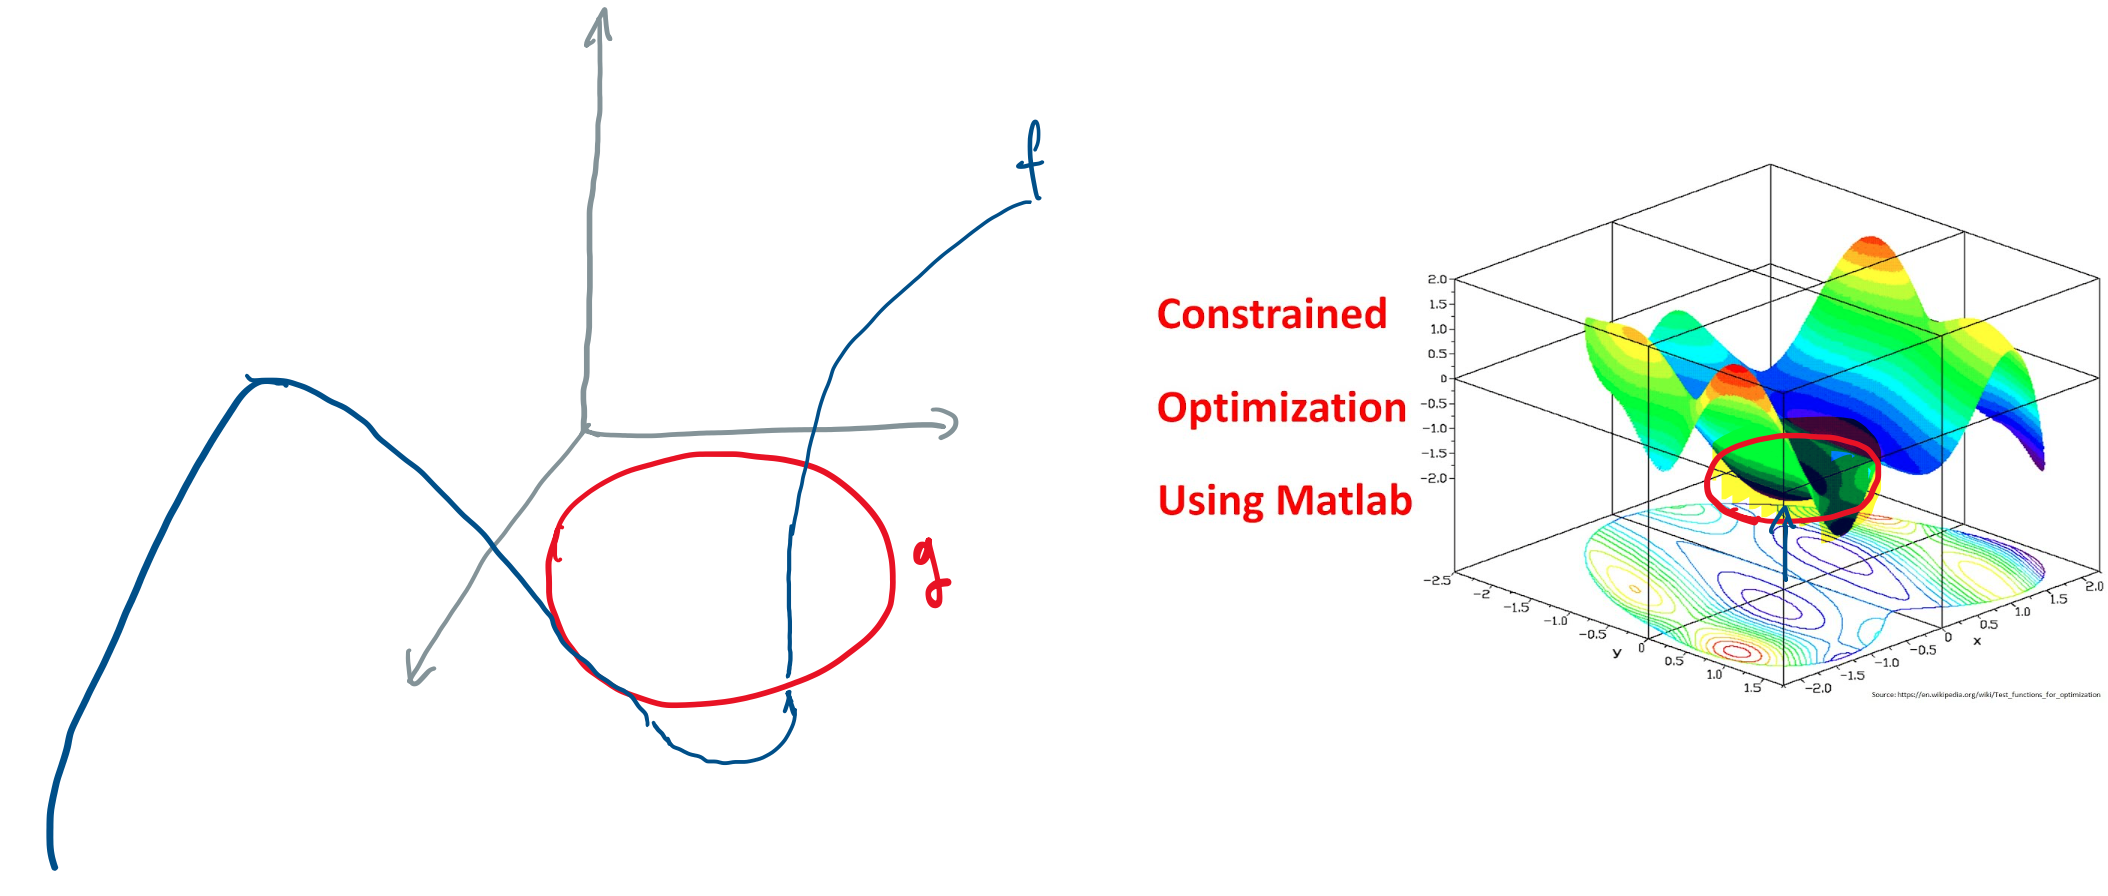
\includegraphics[width=0.5\textwidth]{example.png}
\caption{Blue = function, red = constraint}
\label{fig:ex}
\end{figure}
\noindent
For performing an evaluation of the distance we should integrate the
model, which is computationally expensive. To do one integration we must
perform a lot of computations. Our measure of computational cost is the
number of times we have to simulate the model (per iteration).
\\
\\
\noindent
In most cases, we do not know the gradient, therefore we should
approximate it using the Taylor formula.


\subsection{Gradient approximation with Taylor formula}

$(a,b) \in \mathbb{R}, x_0 \in (a,b)$
\\
\\
\noindent
Let $f_i(a,b) \rightarrow \mathbb{R}$ be differentiable $(n-1)$ times in
$(a,b)$ and $f^{(n)}$ is continuous in $x_0$. Then let $x \in (a,b)$ ,
we have:

$$
f(x)=f\left(x_0\right)+f^{\prime}\left(x_0\right)\left(x-x_0\right)+f''(x_0)\frac{(x-x_0)^2}{2!}+ ...+ f^{(n)}(x_0)\frac{(x-x_0)^n}{n!} + R_n(x) \text{ s.t.} \lim_{x \rightarrow x_0} \frac{R_n(x)}{(x-x_0)^n} =0 
$$
\noindent
We focus on the first terms
$f(x)=f\left(x_0\right)+f^{\prime}\left(x_0\right)\left(x-x_0\right)+R_2(x)=0 \\ f^{\prime}\left(x_0\right)= \frac{f(x)-f(x_0)}{x-x_0}+\left(\frac{R_2(x)}{(x-x_0)}\right)=\frac{f(x)-f\left(x_0\right)}{x-x_0}+R_1(x).$
\\
\noindent
We can also use this trick for $N>1$
\\
\\
\noindent
Let $f: \mathbb{R}^N \rightarrow \mathbb{R}$ and
$e_i=(0, \ldots, 0,1,0,\ldots,0)$.
\noindent
Let's consider $x_1 x+\varepsilon e_i, x-\varepsilon e_i$ ; we are only
moving along one direction.
\noindent
In this case:
$$f\left(x+\varepsilon e_i\right)=f(x)+\varepsilon \frac{\partial f}{\partial x_i}(x)+\frac{1}{2} \varepsilon^2 \frac{\partial^2 f}{\partial x_i{ }^2}(x)+R_3(x) \\ f\left(x-\varepsilon e_i\right)=f(x)-\varepsilon \frac{\partial f}{\partial x_i}(x)+\frac{1}{2} \varepsilon^2 \frac{\partial^2 f}{\partial x_i{ }^2}(x)+R_3(x) \\ \Rightarrow f\left(x+\varepsilon e_i\right)-f\left(x-\varepsilon e_i\right)=+2 \varepsilon \frac{\partial f}{\partial x_i}(x)+R_3(x) \\ \Rightarrow \frac{\partial f}{\partial x_i}(x)=\frac{f\left(x+\varepsilon e_i\right)-f\left(x-\varepsilon e_i\right)}{2 \varepsilon}+R_2(x)$$
\noindent
We have computed an approximation of the first derivative with improved
accuracy.
\\
\\
\noindent
Consider that this only applies to one derivative, we have to perform
this at least twice → 2 function evaluation for each $i \Rightarrow 2W$.
In order to obtain a decent gradient, we require a lot of computations,
but they are fast (quite low number of iterations). We will see other
methods, which are somehow more precise, but also heavier.
\\
\\
\noindent
We can always check $\Delta f=0$ or not to understand if we are done!
\\
\\
\noindent
As we already saw, there might be points where the gradient vanishes
which are not the final destination. Gradient methods may tend to
overfitting, but they are effective. The main issue is that since we
approximate the gradient, we do not trust it everywhere.
\\
\\
\noindent
Gradient methods can be applied to two different categories of problems:

\begin{itemize}
\tightlist
\item
  constrained
\item
  unconstrained

  \begin{itemize}
  \tightlist
  \item
    \textbf{line search algorithm}: follow a direction
  \item
    \textbf{trust region:} create an approximation of the problem
    and solve it in a small trustable region
  \end{itemize}
\end{itemize}


\subsection{Line search}

\subsubsection{Newton's direction}

If we consider Taylor's formula and let $x_k$ be our starting point, let
$\alpha \in \mathbb{R}^+$ step length and $p$ our direction
($x_k, p \in R^n$). For $n=1$, we have:

$$
f(x_k+\alpha p)=f(x_k) + \alpha p f'(x_k) + \frac{\alpha^2p^2}{2} f''(x_k) + r(p^3)
$$
\noindent
For simplicity set $\alpha=1$ and truncate the formula:

$$
f(x_n+p)=f(x_n) + p f'(x_n) + \frac{p^2}{2} f''(x_n) = m_k(p)
$$

→ instead of minimizing the initial $f$, we minimize the simple
polynomial $m_k(p)$.
\noindent
From this equation we can get the direction
$p = -\frac{f'(x_k)}{f''(x_k)}$, which is called \emph{Newton direction}
(best direction). When $n>1$,
$p = -(\nabla^2 f(x_k))^{-1}\nabla f(x_k)$. Finding the inverse of a
matrix is ``a pain'', not straightforward; this is why we will try to
approximate this part.

\subsubsection{Line search algorithm for function minimization}

Set $k=0$ and guess an initial point $x_0$ WHILE $||\nabla f(x_k)||>0$

\begin{enumerate}
\def\labelenumi{\arabic{enumi}.}
\tightlist
\item
  compute $p_k=-(\nabla^2f(x_k))^{-1}\nabla f(x_k)$
\item
  select $\alpha_k$
\item
  update
  $x_{k+1}=x_k+\alpha_kp_k = x_k -\alpha_k(\nabla^2f(x_k))^{-1}\nabla f(x_k)$
\item
  $k=k+1$
\end{enumerate}
\noindent
We stop when the gradient is equal to zero, but we do not really have
zeroes in our computers; therefore, we must apply a threshold
$\varepsilon$.
\\
\\
\noindent
At each iteration we have some issues:

\begin{itemize}
\tightlist
\item
  sometimes we require approximation to compute the inverse of a matrix
\item
  it is computationally expensive to compute all these gradients
\end{itemize}
\noindent
Nevertheless, going in this direction is smart. We can try to tackle the hardest part, i.e.~$p_k$ computation, by
approximation.


\subsubsection{Quasi Newton's direction}

To avoid the computation of $\nabla^2 f$, we build iteratively a
different matrix $B_k$, such that
$B_{k+1}\cdot (x_{k+1}-x_k) = \nabla f(x_{k+1})-\nabla f(x_k)$
{[}condition for the matrix{]}
\\
\\
\noindent
We are approximating the second derivative as second of the gradient.
Since we are already computing the gradient, we exploit it to prevent
extra computations. The difference with respect to standard Newton
direction is the Hessian, which is not computed here.

\textbf{Quasi-Newton direction}:
$P_{k+1}=- \alpha B_{k+1}^{-1} \nabla f(x_k+1)$


\subsubsection{Steepest descent direction}

We proceed in the direction that reduces the gradient the most:

$$
p= -\alpha \frac{\nabla f}{||\nabla f||}
$$
\noindent
In this case we are completely ignoring the second derivative, we only
focus on the gradient computation. This method converges slowly with
respect to Newton and Quasi-Newton's direction.

\hypertarget{selecting-alpha}{%
\subsubsection{\texorpdfstring{Selecting
$\alpha$}{Selecting }}\label{selecting-alpha}}

Ideally, we want to define $\alpha$ s.t.

$$
\bar{\alpha}= \arg \min_{\alpha>0} f(x_k+\alpha p)
$$
\noindent
This is another optimization problem, ideal situation. To avoid solving
the optimization, we usually consider $\alpha$ that satisfies :

$$
f(x_k+\alpha p) \leq f(x_k) + c_1\alpha \nabla f(x_n)^T p_k, c_1 \in (0,1)
$$
\noindent
\textbf{Armijo condition:} the reduction should be proportional to
$\alpha$ and $\nabla f(x_n)^T p_k$.
\noindent
Sometimes thing fails because of parameter choice: it is crucial to
understand why functions fails and how parameters tuning can affect the
most crucial steps in the algorithms.


\subsubsection{Convergence of a method}

The order of convergence of a method (for us) is a constant $\ell$, such
that exists the limit:

$$
\lim_{k \rightarrow \infty  }\frac{||f(x_{k+1})-f(x^*)||}{||f(x_{k})-f(x^*)||^\ell} = L >0
$$

Where $x^*$ is the solution and the method converges.
\\
\\
\noindent
We compare the new iteration (numerator) to the old iteration
(denominator); the limit should go to zero, the exponent is the speed -
the higher the exponent $\ell$, the faster will the upper term go to
zero with respect to the bottom one i.e.~faster convergence. The higher
the exponent, the less iterations are required (in general). For the
methods that we have previously seen:

\begin{itemize}
\tightlist
\item
  steepest descent: $\ell=1$, linear convergence
\item
  quasi-Newton: $\ell \in (1,2)$, superlinear convergence
\item
  Newton: $\ell=2$, quadratic convergence
\end{itemize}

Example: $f(x)=x^4-8x^2+4$

\begin{figure}
\centering
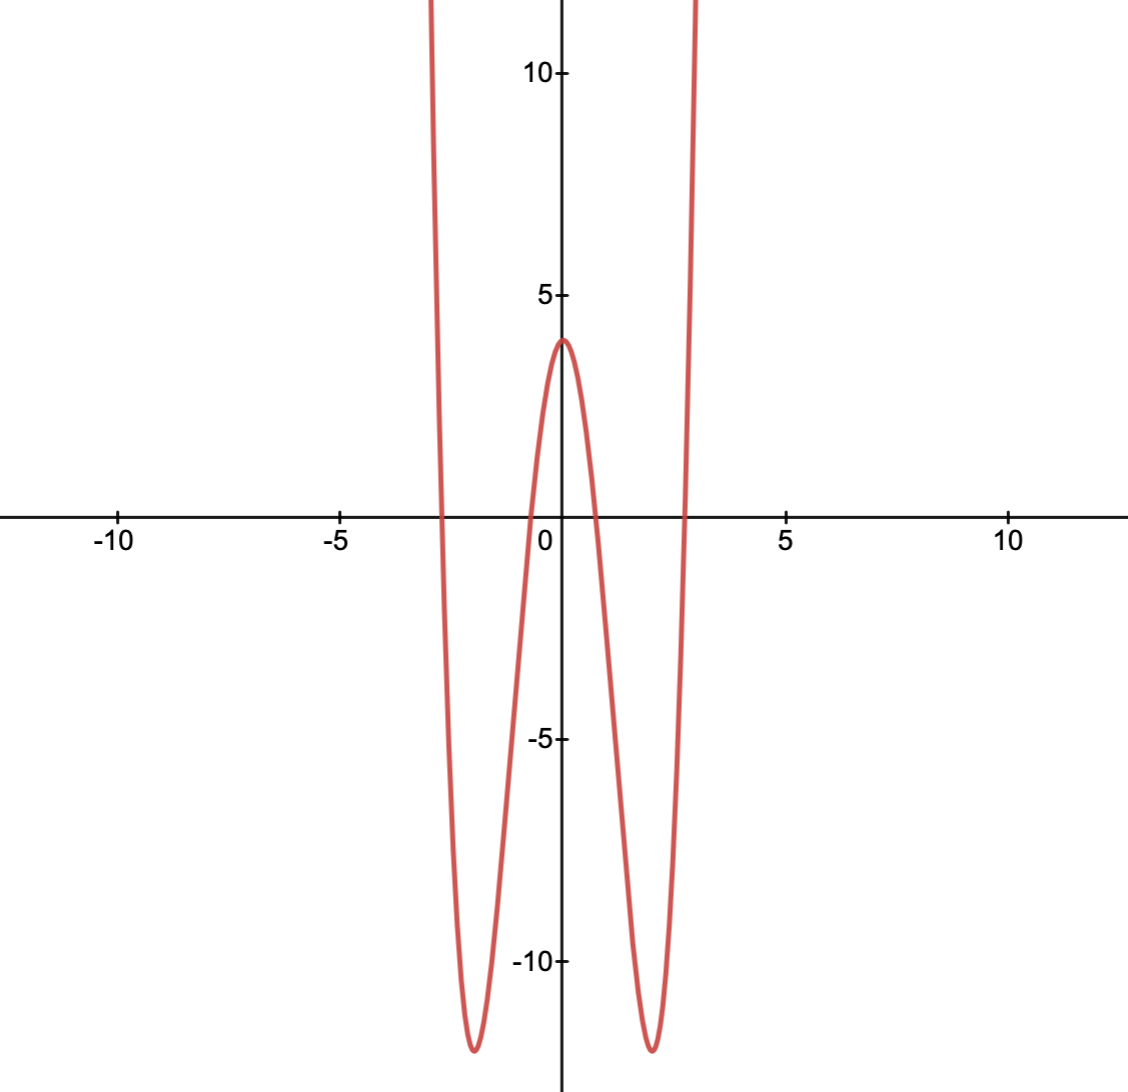
\includegraphics[width=0.3\textwidth]{function.png}
\caption{Desmos  $f(x)=x^4-8x^2+4$}
\end{figure}

$$
x_0=3 \\ f'(x) = 4x^3-16x \Rightarrow f'(x)=0 \Rightarrow  x=0, x=\pm 2\\ f''(x)=12x^2-16
$$

Algorithm: $f'(3)=60, f''(3)=92,$

Let $\alpha=1$:

$$
p_0= -\frac{60}{92}=-0.65 \\ x_1=3-0.65=2.35 \\ f'(2.35) = 14.31\\ f''(2.35) = 50.27 \\ p_1=-\frac{f'(x_1)}{f''(x_1)} = -0.28\\ x_2=x_1+\alpha p_1 = 2.35-0.28=2.07 \\ f'(x_2) = 2.30 \\ f''(x_2)=35.42\\ p_2 = -0.067
$$

Let's try the same by applying Steepest Descent method:

$f'(3)=60 \\ x_1 = x_0..$
$f'(3)=60$
\noindent
In this case the SDM is way faster, lucky shot. But what if we change
the starting point? The direction will always be the same,
i.e.~$p_1 = -1$.

$$
x_1=2.35-1=1.35\\f'(x_1)=-11.75\\x_2=1.35+1 = 2.35 
$$

We are doing ping-pong among two points!
\\
\\
\noindent
The fact that the second derivative progressively shrinks tells us that
we need to reduce the step, but in this case we are not taking this into
account. Of course we also have $\alpha$, we should look at Armijo
condition and change it.
Take into account that each time that we are performing operation on a
number we lose precision.


\subsection{Trust region}

{[}picture{]}
\noindent
Imagine that this is a cut function: our starting point $x_k$ is in the
middle. The main idea of the trust region is that we do not follow a
direction: we approximate the function with a simpler function → Taylor
approximation. According to how big and reliable the approximation is,
we will choose a direction.
\\
\\
\noindent
Last time we approximated the model as:

$$
m(x_p+\alpha p)=f(x_k)+\alpha p^T \nabla f(x_k)+ \frac{1}{2} \alpha^2p^T B_k p
$$

$$
\alpha=1, m_k (p)=f_k+p^T\nabla f_k + \frac{1}{2} p^T B_k p
$$

\hypertarget{trust-region-steepest-descent}{%
\subsubsection{Trust region steepest
descent}\label{trust-region-steepest-descent}}

Define a region such that $||p|| < \delta_k,\delta_k>0$ in which we
solve the optimization problem (1) instead of the original. Remember
that $B_k$ can be the Hessian or an approximation; on the other hand, we
have said that we can also ignore it.
\\
\\
\noindent
Finding a minimum for $m_k(p)=f_k+p^T\nabla f_k$ means that we are
looking for:

$$
\min_p m_k(p)= \min_p (f_k+p^T\nabla f_k)
$$
\noindent
Remember that $f_k$ is a constant, so we want to find a direction for
which $\min_p p^T\nabla f_k$ is minimum. We can rewrite this as:

$$
p^T\nabla f_k = ||p|| ||\nabla f_k|| \cos \theta
$$
\noindent
We minimize for $p$ such that $\cos \theta = -1$ and $||p||=\delta_k$,
where p s.t. $||p|| \leq \delta_k$ {[}radius of the trust region{]}.

$$
\min_p p^T\nabla f_k = -\delta_k || \nabla f_k ||
$$

$$
p = - \delta_k \frac{\nabla f_k}{||\nabla f_k||}
$$
\noindent
This result is exactly the equation from steepest descent. We are
applying a condition on the region with $\delta_k$. This direction and
the whole approach is called trust region steepest descent.
\\
\\
\noindent
We could follow the same idea by applying Newton or Quasi-Newton.
\\
\\
\noindent
To evaluate if we can really trust our region, we define the
\textbf{\emph{actual reduction}} as:

$$
\rho_k = \frac{f(x_k)-f(x_k+p)}{m(x_k)-m(x_k+p)}
$$

By construction $m(x_k+p) \leq m(x_k)$.

\begin{itemize}
\tightlist
\item
  If $\rho_k < 0$ → reject $p$, we are not improving the real problem.
  Usually take $\delta_k = \frac{1}{4} \delta_k$
\item
  If $\rho_k \simeq 1$ → maybe longer step
\end{itemize}
\noindent
$\delta$ value can be tuned according to the needs. The approach is
similar to RK method seen with Marchetti. Of course we have a grey area
between 0 and 1, so we define a threshold e.g.~$\rho_k < \eta$ and
$\rho_k > \eta$.
\noindent
By default, MATLAB uses a trust region algorithm. Having something
certifying that we are doing good or bad is a great thing in
approximation!


\subsubsection{Trust region algorithm}

Let
$\hat{\delta}>0, \delta_0 \in (0,\hat{\delta}), \eta \in (0,\frac{1}{4})$

$k=0, \varepsilon < 0$

REPEAT

obtain $p_k \text{ s.t. } p_k=\arg \min_p m(x_k+p)$

compute $\rho_k$

IF $\rho_k < \frac{1}{4}$

$\delta_{k+1}=\frac{1}{4}\delta_k$

ELSEIF $(\rho_k < \frac{3}{4})$ AND $||p_k||=\delta_k$

$\delta_{k+1}=\min (2\delta_k, \hat{\delta})$

ELSE

$\delta_{k+1}=\delta_{k}$

IF $\rho_k > \eta$

$x_{k+1}= x_{k}+p_{k}$

ELSE

$x_{k+1}= x_{k}$

IF $||\nabla f(x_{k+1})||<0$

BREAK
\\
\\
\noindent
We stop if the gradient is sufficiently small. Our focus is on computing
$p_k$. We then evaluate $\rho_k$ to adjust parameters (which is simpler
from what we have previously seen).
\\
\\
\noindent
If we apply this algorithm to the example of last lecture, it happens
that with $x_0=235$ and steepest descent $\rho_0=0.17 < \frac{1}{4}$,
which tells us to reduce $\delta$. The only thing that changes is $\rho$
changes.
\\
\\
\noindent
PROBLEM:

$$
g(x,y)=x^4+y^4+xy
$$

\url{https://www.benfrederickson.com/numerical-optimization/} play with
learning rate, explore the site.


\section{Least squares problems}

Recall that if $m$ is the model, we quantified the distance between the
model output and data as:

$$
m_j(t_i,(x_0,t_0), \theta) = m_{ij}(\theta) - \hat{y}_{ij}, \text{for } i,j \text{ as lesson 2 } 
$$

$r_{ij}(\theta)$ is called RESIDUAL and we shape it as a vector.

$$
J_k=J(\theta_k)[\frac{\partial r_I}{\partial\theta_i}], i=1, ...,n, I=1,...n
$$
\\
\\
\noindent
Since the time points are given by the data, everything only depends on
the choice of parameter theta, which is a vector of parameters. We can
derive the residual according to theta. Our function to minimize is
$f(\theta)=\frac{1}{2}\sum^m_{j=1}r_j^2(\theta)$
\noindent
It will hardly go to zero, as our observations are affected by noise: we
just need to explain data, not noise. If we have the distance of the
single point we can see the effect of each parameter by looking at the
derivative. Here we have that the gradient (Jacobian) will be telling us
the relationship among model parameters and data.

$$
\nabla f(\theta)=\sum^m_{j=1}r_j(\theta)\nabla r_j(\theta)= J(\theta)^Tr(\theta)
$$
\noindent
The matrix notation is a more convenient way to express this gradient.
While solving least squares problems we always exploit Taylor
approximation.

Hessian matrix:

$$
\nabla^2 f(\theta)=J^T(\theta)J(\theta)+ \sum^m_{j=1}r_j(\theta) \nabla^2 r_j(\theta)
$$
\noindent
What's \emph{magical} of this is that we can use $J^T(\theta)J(\theta)$
as approximation for $B(\theta)$ of our gradient.

If the problem is linear, $r(\theta)=A(\theta)-y$. The objective
function $f(\theta)=\frac{1}{2} || A\theta-y||^2$ and
$\nabla f(\theta)=A^T(A\theta-y), \nabla^2 f(\theta)=A^TA$.

If $f$ is convex
$\Rightarrow \exists \theta^* s.t. \nabla f(\theta^*)=0 - A^TA\theta^*=A^Ty$
\\
\\
\noindent
We reach a normal equation, linear system (we know how to solve this). With general functions, this is not so straightforward; what we will do
is approximating the problem with a solvable linear problem.
\\
\\
\noindent
When we try to quantify the distance between the model and our points we can formalize the problem as:

$$
r_i = m_i(t,\theta) - y_0 \\ f(\theta)= \frac{1}{2} \sum^m_{j=1} r_j^2 (\theta) \\ \nabla f(\theta) = J(\theta)^{T} r (\theta) \\ \nabla f(\theta) = J(\theta)^{T} J (\theta) + \sum^m_{j=1} r_j \theta \nabla^2 r_3 \theta\\
$$
\noindent
Last time we already said that we will ignore the sum, for two reasons:

\begin{enumerate}
\def\labelenumi{\arabic{enumi}.}
\tightlist
\item
  it contains second order derivatives, painful to compute
\item
  the Newton direction is a quasi vector
\end{enumerate}

So at every iteration $k$ we solve the approximated problem

$$
J(\theta_k)^TJ(\theta_k)p=-J(\theta_k)r(\theta_k) \\ J_k^TJ_kp=-J_k^T r_k
$$
\noindent
This is a linear system which we can solve. In this case, we are
solving:

$$
f(\theta_k+p)= \frac{1}{2} ||r(\theta_k+p)||^2 \simeq \frac{1}{2} ||J_kp+r_k||^2
$$
\noindent
This is what we called normal equation for a normal least squares
problem. Under certain hypotheses the method converges quadratically!
\\
\\
\noindent
We discussed last time that Newton is quadratic convergent. Of course
the matrix should not be singular, we need to be able to solve the
system. We start with a problem in a special form, sum of squares.
Thanks to this, we can rewrite the problem in a simpler way and perform
an approximation, leading to solving a linear system at each iteration.
This approximation guides us rapidly to a solution. We are applying
linear search, by defining a direction and solving a new problem at each
iteration. The biggest issue could be the non invertible matrix, but we
can do something to circumvent the issue.


\subsection{The Levenberg-Marquardt method}

At each iteration, we solve the problem:

$$
\min_{||p||\leq\delta_k} \frac{1}{2} ||J_kp-r_k||^2
$$
\noindent
We can have a solution inside the trust region $\delta_k$ or on the
border i.e.~not the minimum, but the smallest value we can reach.

\begin{itemize}
\item
  case 1: $\beta$ is a solution and $||p||\leq\delta_k$ → DONE
\item
  case 2: $||p||=\delta_k$ , then $\bar{p}$ is a solution if and only if
  $\exists \lambda > 0$:

  $$
    (J^TJ-\lambda I)=-J^Tr \\ + \lambda(\delta_k-||p||)=0
    $$
\end{itemize}
\noindent
If we can push it a bit further from zero and the problem is still
solved, we can think of it as a solution. If we are hitting the boundary
$\lambda(\delta_k-||p||)=0$, we want to move the matrix a bit from
singularity. We will not use it very much, but it is a well known
algorithm. It is one of the default MATLAB solvers. The
Levenberg-Marquardt converges quadratically when we are close to the
solution, while if the residuals are big it does not perform well.


\subsection{Solving a problem with bounds}
We have seen together that we can exploit the Lagrangian for the
  equality constraint, but we can have other boundaries. There are other
  approaches which allow us not to lose our approximation advantage. We
  can simply do \textbf{\emph{variable transformation}} : instead of
  changing the problem, we change the variables.
\noindent
Example: $x \rightarrow e^x, \mathbb{R} \rightarrow \mathbb{R}_0^?$
{[}other example missing, cannot understand from recording{]}
\\
\\
\noindent
 Another solution could be to include the bound in the \textbf{\emph{trust region}}.

{[}drawing missing{]}
\noindent
\emph{Evolutionary algorithms} follow the evolution of the solution: at
the beginning look for solutions, then add a penalty for the boundaries.

\subsection{Solving global minimum problem}

How can we be sure that we are looking at a global minimum? We can start
from another initial point and check whether the solution reaches the
same minimum.
\noindent
From local to global → the \textbf{\emph{multi-start approach,}} t is a
shortcut, but the best way to work.

\subsection{Gauss-Newton method}

Let $N \in \mathbb{N}, \varepsilon > 0, J$ as defined before. We randomly select N vectors and use
$\theta^1, \dots, \theta^n \in \mathbb{R}^n$

For each $i=1,\dots,N$ DO

REPEAT

$\bar{J}=J(\theta^i)$

compute $q$ s.t. $\bar{J}^i\bar{J}q=-\bar{J}r(\theta^i)$

compute $\vartheta = \theta^i + q$

compute $\varepsilon = ||\frac{\theta^i-\vartheta}{\theta}||$,
\emph{relative increase}

update $\theta^i = \vartheta$

IF $\varepsilon<\bar{\varepsilon}$ then BREAK

SAVE $\theta^i$

END

→ no global minimum guarantee!
\\
\\
\noindent
There are other ways to detect if a minimum is global e.g.~we try to
divide the space in N different sectors and pick points for each one of
them, \emph{Latin hypercube} and \emph{orthogonal sampling}. The more we
do it, the more we acquire confidence, but we will never be sure. In
addition, we always have to deal with noise, we do not know if the
minimum is the best or we are overfitting.
\\
\\
\noindent
Example on MATLAB: if we take only 10 random points we can have a biased
result. By taking a bigger sample, we should somehow achieve a fuller
result in the region. Still, we have some holes and repeated points. Are
there smarter ways to take random points?


\subsection{Latin hypercube sample}

Get random numbers dividing the interval in m sectors. This is a 2x2
problem and we need to reason on some aspects: if we take the square
(0,1),(0,1) out of 100 points we will just have 3/4 there → not
exploring it very well. If parameters are between 0.1 to 1000 we need to
better sample.

$n = 20$, the fewer points we get, the more we see the difference among
the two methods.

$n = 200$, still we have missing parts.

$n = 2000$, thousands of iterations → if we zoom in there is still a lot
of space
\\
\\
\noindent
The takehome message is that it is almost impossible to cover all the
space with points. Luckily these are starting points, if they are close
to the solution we will have the good direction. Gradient methods are
expensive, but they are smart.


\subsection{MATLAB}

When an optimizer stops, it gives as output the function converged to
the solution or why it stopped. Termination criteria: gradient,
incremental step e.g.~is our step too small?, change in x was less of
certain tolerance, the residual was less than specific tolerance, max
number of iterations. These conditions are added in order to avoid
infinite function evaluation.
\\
\\
\noindent
We first need to define an enzymatic reaction as a set of ODEs. We then
specify initial concentrations and a given set of rates. Integrate the
model and plot the simulation results.
\\
\\
\noindent
The dots are the experimental points, lines are the output of the
simulation. According to different starting points, we will obtain
different results; we need to quantify how much the model is distant
from the real data. The output of the normal simulation is a set of
points; we can do a linear interpolation for time and values, giving how
much is each of the simulated variables at the requested time. Once we
have the values at the right time, we can compute the \emph{residuals}
through the sum of squares. In some cases we can also look at weighted
residuals and normalize them; however, zeros are problematic → our
experimental data goes to zero, we stick to normal SSE.
\\
\\
\noindent
Our objective function takes the rate, experimental time and values,
initial and final time. We call the solver (15s as the system is stiff,
we require a more robust iteration) and get a vector of residuals and
SSE.
\\
\\
\noindent
If we compute the residual with $s_1$,$s_2$ and $s_3$ we can easily understand
which is the better one (matches visual inspection of the plot).
\\
\\
\noindent
We can then optimize and find the solution with \texttt{lsqnonlin}
e.g.~$SSE1 = 33.6653$, $resNorm = 38$, worse, we should improve initial
conditions.

{[}Recap from last time{]}
\\
\\
\noindent
\textbf{MATLAB multi-start} is a wrapper working with different
algorithms. It will automatically parallelize the problem. It requires
to insert starting points and tolerance. We therefore define bound,
create problem and give initial points e.g.~lsqnonlin + objective
function. The output contains the result of parallel lsqnonlin and
parameters, somehow similar to what we saw before. We can reduce the
bounds, but solution 1 is still the best. Main limitation: heavily
depends on the number of initial points.

\begin{figure}
\centering
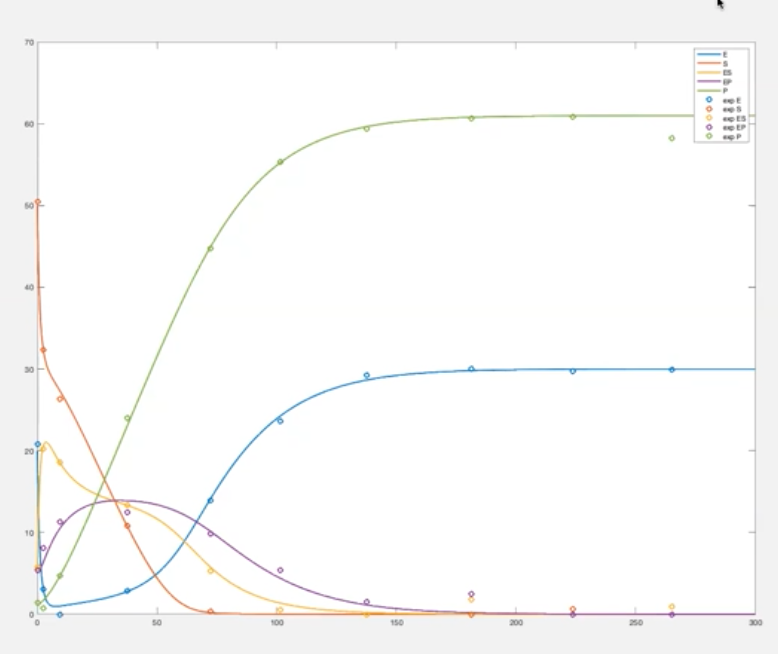
\includegraphics[width=0.45\textwidth]{multistep.png}
\caption{MATLAB multi-start lsqnonlin}
\end{figure}

\noindent
Remarks:

\begin{itemize}
\tightlist
\item
  we did a lot of computations
\item
  $s_1$, the initial set of parameters, had values at different orders
  of magnitude. We really do not know if we are doing well or not.
\end{itemize}


\section{Stochastic methods for parameter estimation}

Stochastic methods are often used when we cannot compute the gradient.
With the same parameters, stochastic methods can produce dramatically
different results.

\begin{figure}
\centering
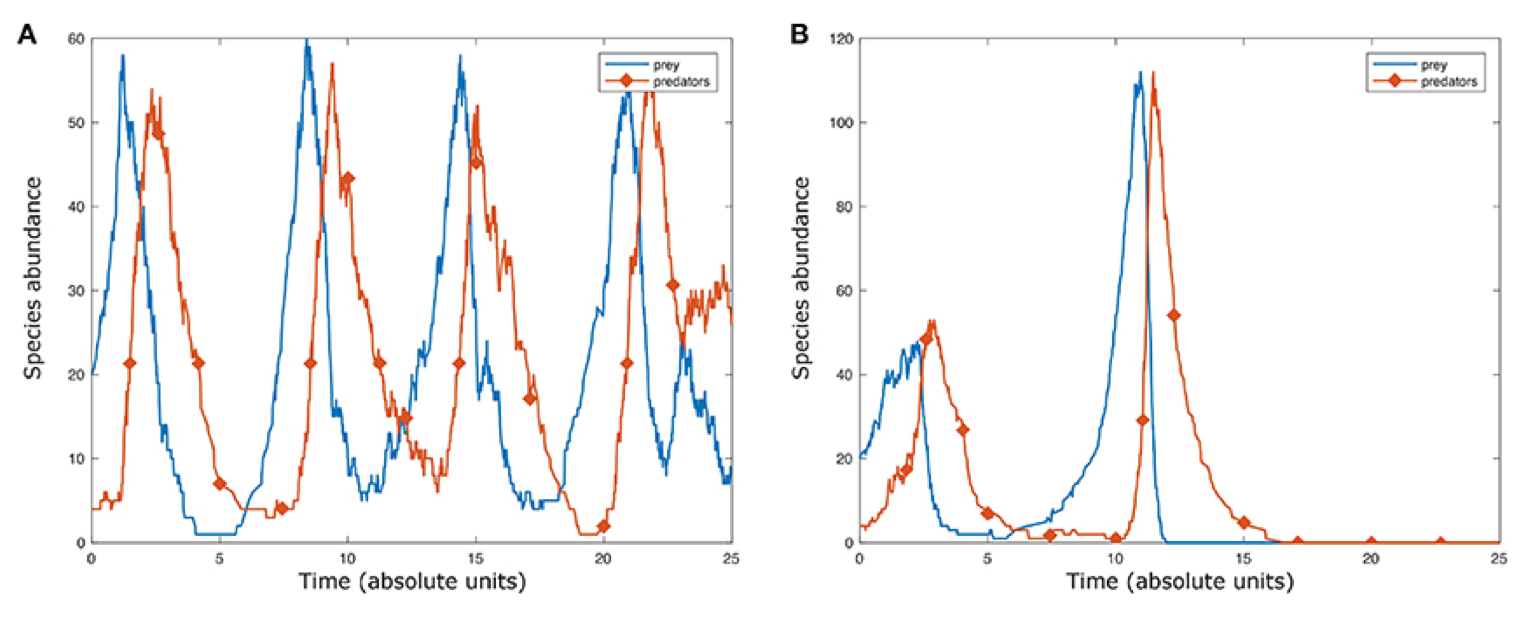
\includegraphics[width=\textwidth]{stoch_LV.png}
\caption{Lotka-Volterra stochastic simulation results. In B we witness
preys and predators extinction, it is the output of a simulation
performed with the same model and parameters as A.}
\label{fig:res}
\end{figure}

Lotka-Volterra stochastic simulation results are reported in Figure \ref{fig:res}- In B we witness preys and
predators extinction, it is the output of a simulation performed with
the same model and parameters as A.
\\
\\
\noindent
Instead of following the gradient, we collect information in a manner
resembling natural selection. Monte Carlo Methods are dated around 1949,
the name comes from casinos (recalls concept of luck). In order to use
MCM to do inference, Metropoli and Hastings developed a specific
algorithm in 1970.


\subsection{Markov Chain Monte Carlo (MCMC)}

MCMC is a chain of events where the current state depends on the
previous one and on the transition probability.
\noindent
If $x^{(i)}$ is a random variable (stochastic process) and it takes only
discrete values $\{x_1,\dots,x_s\}$. Let $p(x)$ be the probability
distribution of $x$. $x^{(i)}$ is a Markov Chain if:

$$
p(x^{(i)}|x^{(i-1)},\dots,x^{(1)})=T(x^{(i)}|x^{(i-1)})
$$
\noindent
Simplest case: a MC is \textbf{homogenous} if $T(x^{(i)})x^{(i-1)}=T$,
i.e.~the transition matrix is constant.
\\
\\
\noindent
If we run MCMC long enough, they will hopefully reach a stable point.
\\
\\
\noindent
Example: 3 states and homogenous transition matrix

$$
T = \begin{bmatrix}
0 & 1 & 0\\
0 & 0.1 & 0.9\\ 0.6 & 0.4 & 0\\
\end{bmatrix}
$$

\begin{figure}
\centering
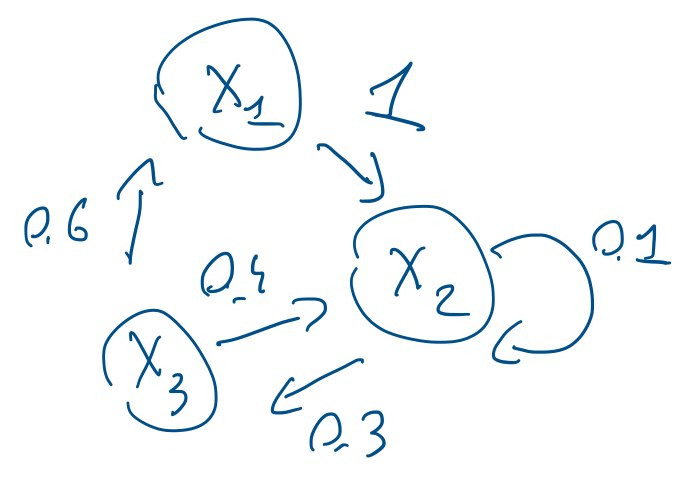
\includegraphics[width=0.3\textwidth]{mcmc.png}
\caption{MCMC example}
\label{fig:MCMCexample}
\end{figure}

MCMC example (Figure \ref{fig:MCMCexample}):

$$
\pi_1=\begin{pmatrix}0.5 & 0.2& 0.3 \end{pmatrix}
$$
\noindent
The next probability of being in the three states is given by

$$
\pi_1 \cdot T=\begin{pmatrix}0.3\cdot0.6, & 0.5+0.02+0.12,& 0.18 \end{pmatrix} = \begin{pmatrix}0.18, & 0.64,& 0.18 \end{pmatrix}
$$
\noindent
If we do this enough, we will always arrive to a fixed distribution,
called invariant distribution $\Rightarrow$ we want to build a Markov
Chain whose invariant distribution is the distribution of our unknown
parameters.

$$
p(x)=\dots = \begin{pmatrix} 0.2213 \\ 0.4098 \\ 0.3689\end{pmatrix}^T
$$
Where p(x) is called \textbf{invariant distribution}.
\\
\\
\noindent
A stochastic matrix is \emph{irreducible} if its graph does not contain
unconnected sub-graphs. If T is an irreducible transition matrix (+ aperiodic) → the MC has an
invariant distribution.
\noindent
We must connect probability distribution / values for the parameters
with the model. There is a known function that we can use to do so.
\\
\\
\noindent
Monte Carlo refers to a family of methods developed for
\textbf{sampling}. In particular, we obtain samples of a certain i.i.d.
random variables $\{x^{(i)}\}_{i>0}$ from a known density $p(X)$.
\\
\\
\noindent
The samples can be used to ``estimate / approximate'' a target density /
distribution. We exploit known distributions e.g.~Normal,
Poisson,\ldots{} to approximate our unknown distribution of interest.
\\
\\
\noindent
Given enough samples, we can approximate $p$ as:

$$
p_N(x)= \frac{1}{N}\sum^N_{i=1}\delta_{x^{(i)}}(x)
$$

with
$\delta_{x^{(i)}}(x)= \begin{cases}1, & x=x^{(i)} \\ 0, & \text{elsewhere}\end{cases}$
\noindent
This is often used to approximate ``hard'' integrals. We can approximate
and integral with a finite sum of values, which is obtained as:

$$
I_N(f)=\frac{1}{N} \sum^N_{i=1} f(x^{(i)})
$$
\noindent
Here we are evaluating the function is some points. We can use the mean
as an approximation of the integral. This equation converges to the real
integral by the law of large numbers.

$$
I_N(f)=\frac{1}{N} \sum^N_{i=1} f(x^{(i)})  \xrightarrow[N \rightarrow \infty  ]{}   I(f)= \int_x f(x)p(x)dx
$$
\noindent
A probability is richer than the output of one least squares, we have
information on the shape.


\subsection{Sampling a distribution}

Let $p$ be a known probability distribution (up to a proportionality
constant). We usually prefer to sample from a well-known distribution
$q(x)$ s.t. $\exists M>0$

$$
p(x) \leq M q(x)
$$


\begin{figure}
\centering
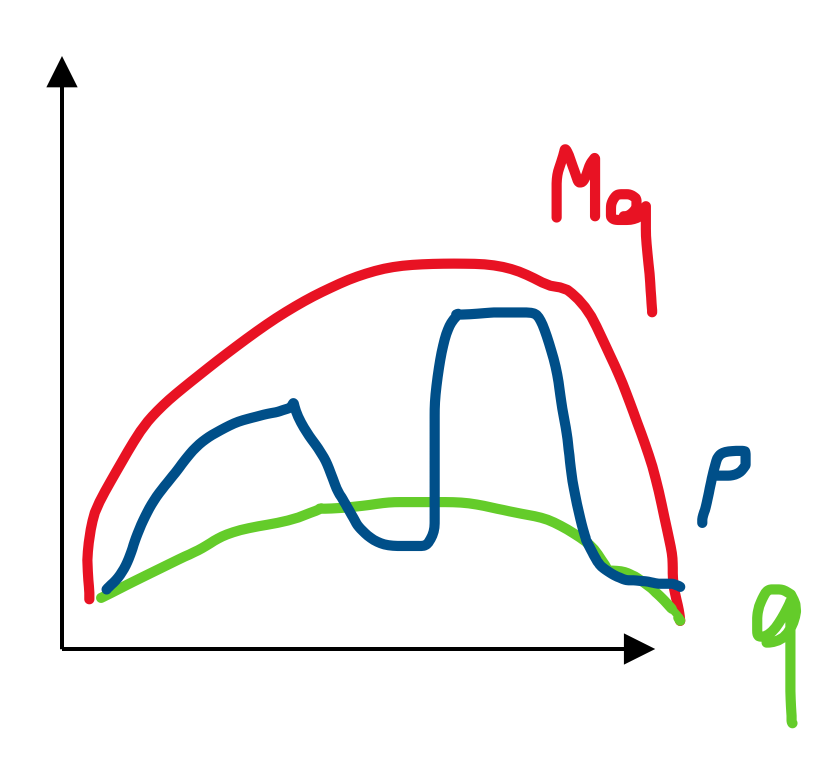
\includegraphics[width=0.3\textwidth]{distribution.png}
\caption{Example: bimodal distribution}
\end{figure}
\noindent
We extract values from $q$ if they are smaller than $Mq$; each time we
are collecting information on $p$ collecting from $q$.

\subsection{Rejection sampling algorithm}

Set $i=1$

REPEAT

Sample $x^{(i)}$ from $q$ and $u \in \mathcal{U}(0,1)$

IF $u < \frac{p(x^{(i)})}{Mq(X^i)}$ and $x^{(i)}$

$i=i+1$

ELSE

REJECT
\\
\\
\noindent
If the point is in the area between p and Mq we still accept it; the
further the ratio is from one, the smaller the chance of keeping the
point.
\\
\\
\noindent
At this point we are using a known distribution $p$; we then gradually
remove what we know in the following iterations.


\subsection{Metropolis Hastings}

Let $X$ be our current point, $q$ the proposal distribution and $p$ the
target distribution. $p$ can be an unnormalized density
($\int p > 1 \text{ but} \int p < \infty)$. Ideally we want to know $p$,
but if it is unknown we can still proceed. Let us call this function $h$
(non negative and positive integral).
\\
\\
\noindent
$X^*$ is the new candidate point. The trick of MH algorithm is to avoid
relying on probability, we use a function. We require info on $p$, but
not a probability.

\textbf{Metropolis ratio} $r_M(x,x^*)=\frac{h(x^*)}{h(x)}$

\textbf{Hastings ratio}
$r_H(x,x^*)=\frac{h(x^*)\cdot q(x^*|x)}{h(x)\cdot q(x|x^*)}$
\noindent
From the distribution, we want to measure how likely the previous value
is based on the current value. We are weighting our choices to
likeliness.


\subsubsection{MH algorithm}

Guess $x^{(i)}$

FOR $i=0$ to $N-1$

Sample $x^*$ from $q(\cdot|x^{(i)})$ and $u \in \mathcal{U}(0,1)$

IF $u < \min \{1, r_H(x,x^*) \}$

$x^{(i+1)}=x^{(*)}$

ELSE

$x^{(i+1)}=x^{(i)}$

END

END
\\
\\
\noindent
We sample from a proposal distribution and accept according to another
function i.e.~if it is more likely. If it is not more likely, we accept
it with a certain chance.
\\
\\
\noindent
MATLAB plot:

\begin{itemize}
\tightlist
\item
  right: histogram with the known distribution
\item
  left: MCMC oscillating between 0 and 10, recapitulates the
  distribution
\end{itemize}
\noindent
The procedure is really fast, takes less than a second. If instead of
extracting u and v from random distribution with an index, the result is
the same → ``thanks MATLAB, it is not necessary to prelocate anymore''
\\
\\
\noindent
If we employ a Gaussian distribution, the result is still good but not
as accurate as the previous one. We are adding complexity by introducing
the variance; by choosing a different value we can improve the result.
Pay attention to the fact that if we sample from a narrow distribution,
we risk focusing only on one of the two points.
\\
\\
\noindent
Everything we do has consequences!


\subsubsection{Visualization of MCMC}

\url{http://chi-feng.github.io/mcmc-demo/app.html?algorithm=RandomWalkMH\&target=banana}
\noindent
Green: accept, red: reject
\\
\\
\noindent
\underline{Target distribution = standard}

\begin{itemize}
\tightlist
\item
  GibbsSampling: collects points according to a certain direction from a
  starting point, it tries to rebuild a 2D Normal distribution.
\item
  AdaptiveMH: sample from a starting mean and accept or reject new
  points.
\item
  Random walk: more or less like MH. Even if the target distribution is
  not that difficult (bell shape), there are a lot of rejections
  initially.
\item
  DE-MCMC-Z: produces vectors.
\end{itemize}
\noindent
\underline{Target distribution = donut}

\begin{itemize}
\tightlist
\item
  SVGO: stochastic vector gradient descent, intermediate between
  gradient and stochastic.
\item
  EfficientNUTS (No-U-Turn samples): it creates many points, more
  complex but one of the best. In the end it will converge quite fast.
\item
  RandomWalk: needs more time to converge with respect to standard
  distribution.
\end{itemize}
\noindent
\underline{Target distribution = multimodal}

\begin{itemize}
\tightlist
\item
  RandomWalk: three initial points, it proposes a random perturbation.
\item
  AdaptiveMH: changes some of the parameters. Differently from the
  previous approach, the shape changes: instead of having a fixed search
  area, it evolves and adapts.
\end{itemize}


\subsubsection{How to link data and MH}

In LSQ, we used the function

$$
f(\theta)=\frac{1}{2}\sum^m_{j=1}r^2_j(\theta)=\frac{1}{2}\sum^m_{j=1}(y_j-m_j(t_i,\theta))^2
$$
\noindent
We can weight our residuals for their uncertainty:

$$
f_w(\theta)=\frac{1}{2}\sum^m_{j=1} \frac{r^2_j(\theta)}{\vartheta_j^2}
$$
\noindent
$\vartheta_j$= (for example) the standard deviation of that measured
point.
\\
\\
\noindent
We can use as function to link the parameters and the output, and be
non-negative: {[}where $Y$ is the vector of our observations{]}

$$
L(\theta|Y)=\exp(-f_w(\theta)) \geq 0
$$
\noindent
We can use this as $h$ in the MH algorithm.
\\
\\
\noindent
Metropolis ratio:

$$
r_H(\theta^*,\theta)=\frac{L(\theta^*)}{L(\theta)}=\frac{e^{-f_w(\theta^*)}}{e^{-f_w(\theta)}}=\exp(-f_w(\theta^*)+-f_w(\theta))
$$
\noindent
So since $f_w(\theta)\geq0$ we have that if
$f_w(\theta^*) > f_w(\theta) \Rightarrow r_H>1$ , we ACCEPT. Otherwise
we accept with a certain probability. This kind of function can be used
to link the new parameters with data.
\noindent
We can work with log-likelihood also here, we just look at
$f_w(\theta^*)$ and $f_w(\theta)$.


\subsection{Random walk MCMC}

Let us assume $\theta^*$ is sampled from
$\mathcal{N}(0,\mathcal{C})+\theta=\mathcal{N}(\theta,\mathcal{C})$
\\
\\
\noindent
We add a perturbation with $\mathcal{C}$, a known covariance matrix.
$\mathcal{C}$ can be fixed or adapted along the iterations.
\\
\\
\noindent
From the initial point we have a new candidate according to a
multivariate normal distribution; if the candidate is accepted, we we
will then restart evaluation from it. We are collecting some information
allowing us to shape the target distribution.


\subsubsection{Algorithm RW-MCMC ( C known)}

Initialize a matrix $D_\theta$ and a vector $V_L$

Randomly generate $\theta_1$

Compute $L(\theta_1)=L_1$

For $i=1:N$

	sample $Z \sim N(D,\mathcal{C})$

	compute $\theta_2=\theta_1+Z$

	compute $L_2=L(\theta_2)$

	compute $\text{ratio}=\frac{L_1}{L_2}$

	sample $u \sim\mathcal{U}(0,1)$

	IF $u < \text{ratio}$

		$L_1=L_2$

		$\theta_1=\theta_2$

	END

	IF $i > \text{warm-up}$

		$D_\theta=[D_\theta;\theta_1]$

		$V_L=[V_L;L_1]$

	END

END
\\
\\
\noindent
We want to find a good accept-reject tradeoff to reach a satisfactory
convergence.
\\
\\
\noindent
\textbf{Pros}

\begin{itemize}
\tightlist
\item
  the object function is evaluated once per iteration
\item
  the target distribution can be built form the samples
\item
  we only need the last point to restart
\item
  we can collect info on the model: variability on the output +
  sensitivity on parameters
\item
  random selection helps us to avoid local minima
\end{itemize}

\noindent
\textbf{Cons}

\begin{itemize}
\tightlist
\item
  convergence may be slow
\item
  sampling distribution may affect the results
\item
  each MCML cannot be parallelized
\item
  burn-time
\item
  diagnostics are heuristics
\end{itemize}


\subsubsection{Diagnostics}

We can exploit diagnostics to check if the parameters are good and
understand whether we are done or not.

\begin{enumerate}
\def\labelenumi{\arabic{enumi}.}
\tightlist
\item
  chain 1: expected MCMC plot
\item
  chain 2: we require a longer burn-in, we have not reached the target
  distribution
\item
  chain 3: we do not have enough information, the number of iterations
  is too small
\end{enumerate}

\begin{figure}
\centering
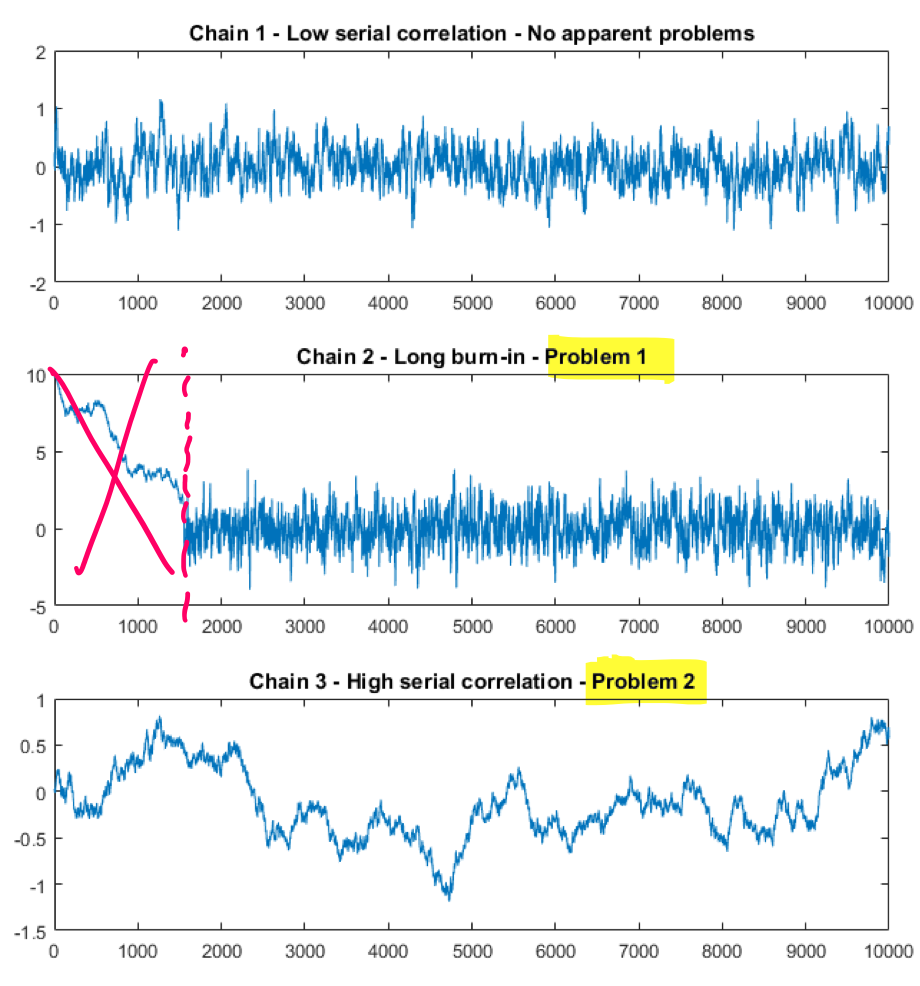
\includegraphics[width=0.5\textwidth]{diag_1.png}
\caption{Diagnostic 1}
\end{figure}
\noindent
The desired output of MCMC should look like the following plots:

\begin{figure}
\centering
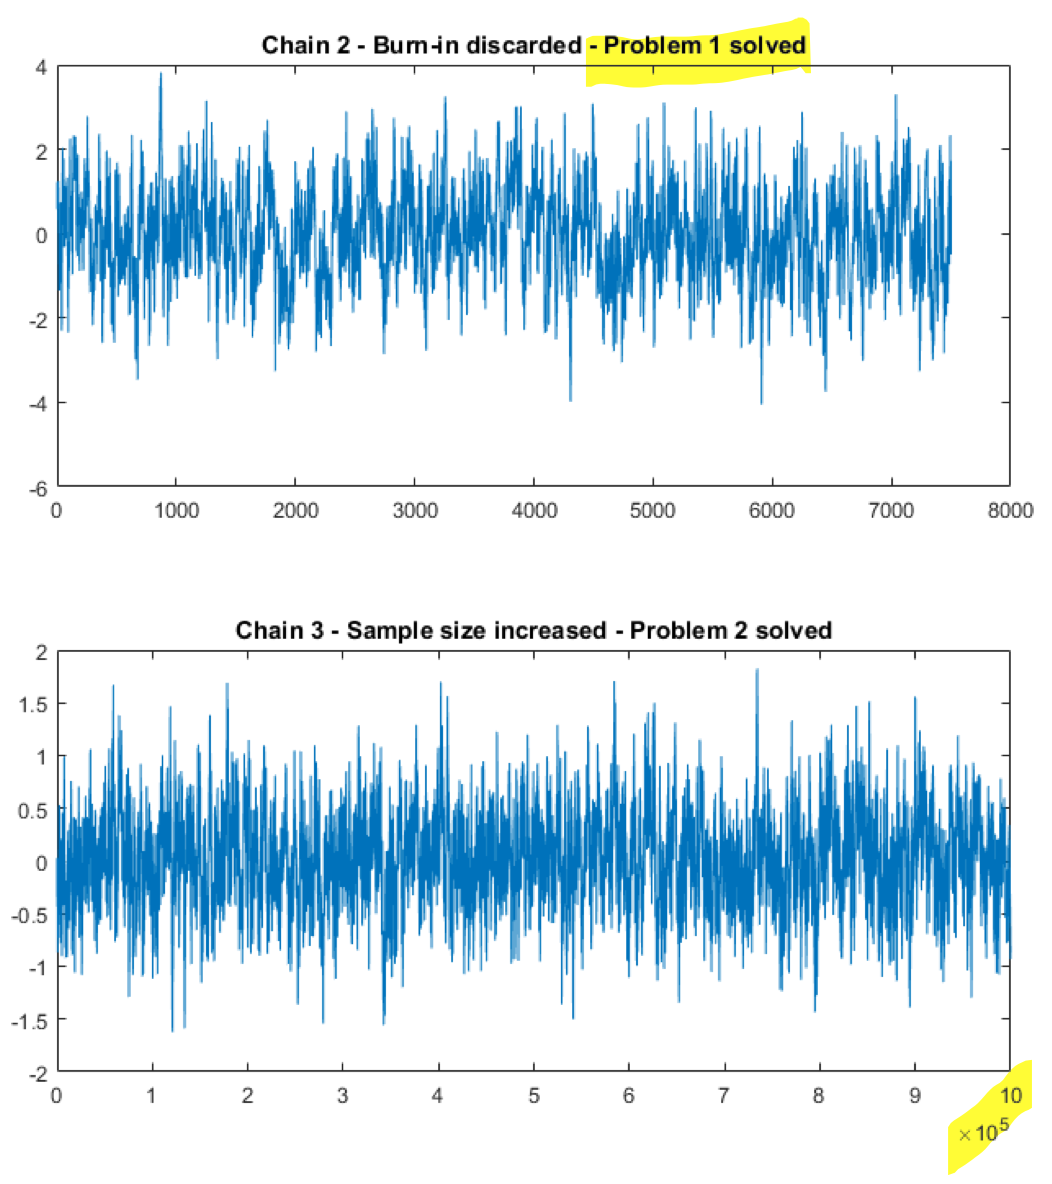
\includegraphics[width=0.5\textwidth]{diag_2.png}
\caption{Diagnostic 2}
\end{figure}

\noindent
Another more analytical approach is \textbf{sample split}. If we split
the plot in different regions, do they have the same mean? Do we observe
consistency? In chain 2 we need longer warm up, in 3 we need more
samples.

\begin{figure}
\centering
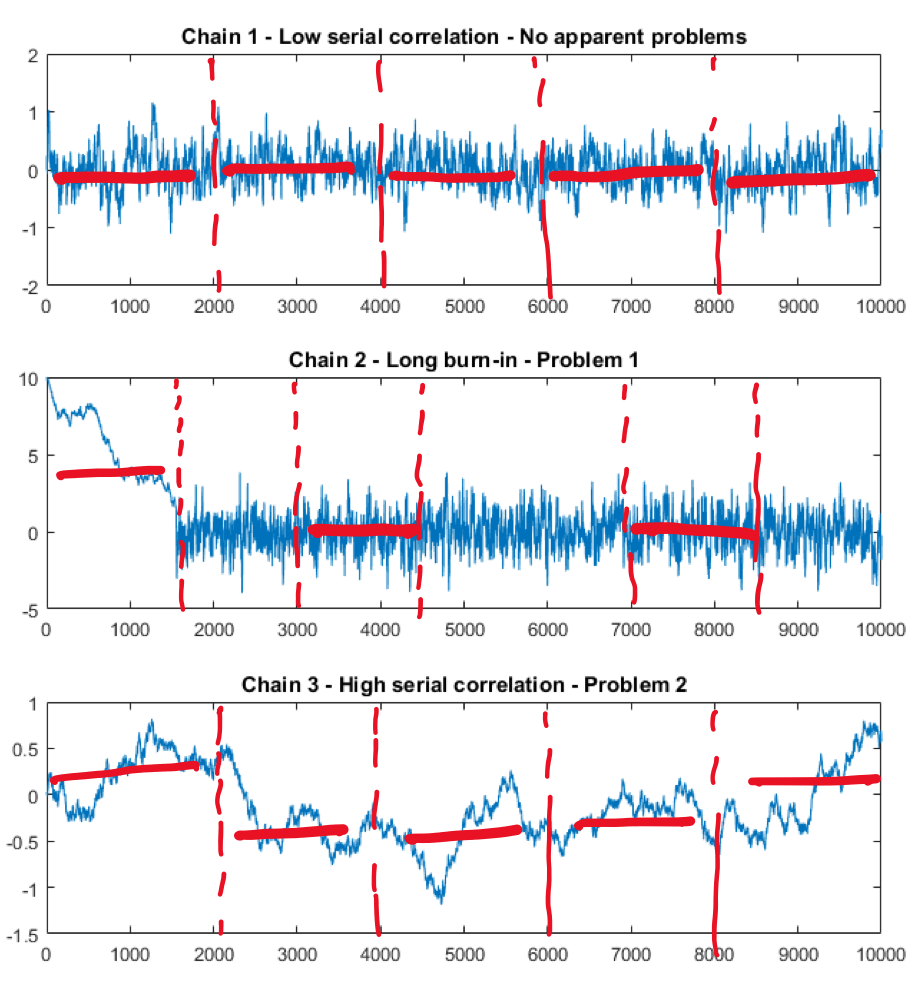
\includegraphics[width=0.5\textwidth]{diag_3.png}
\caption{Diagnostic 3}
\end{figure}
\noindent
Differently from gradient methods, here things are a bit more hard to
interpret. We know that eventually we will reach oscillations around the
global optimum, but we have no guarantee.
\\
\\
\noindent
Diagnostics are based on the observation of the results, so they might
be biased by our belief and they do not provide an easy way to read
``certificate'' of convergence.
\\
\\
\noindent
Another approach may be run more MCMC in parallel and see if they all
converge to the same distribution. However, it is again not a
certificate of convergence to the global optimum.
\\
\\
\noindent
Last observation: constraints and bounds can be included easily in the
proposal distribution or in the likelihood.

\section{Heuristics and the genetic algorithm}

``Heuristics is a fancy name for trial-and-error''.

Heuristics mimic natural selection i.e.~follow nature inspired
procedures. At the growing of computational power, they become feasible
ways to solve optimization problems. There are no warranties on the
exactness of the solutions, but often times the results are of high
quality. In addition, heuristic algorithms are easy to implement, are
general and can include \emph{constraints} (even complex ones).
\\
\\
\noindent
Example: timetable for plane departures. Deciding when a plane lands is
not only a function of flight time, we should take into account delays,
passengers, luggages, crew, \ldots{} → constraints. In biological
problems we can include relationship among variables which should be
satisfied, allowing high flexibility.

There are many famous heuristic algorithms:

\begin{itemize}
\tightlist
\item
  simulated annealing: used in physics, match thermal dispersion
\item
  ant colonies: ant are able to solve many problems e.g.~supply chain
\item
  covariance matrix adaptation evolution strategy: performs similarly to
  adaptive MH algorithm
\end{itemize}
\noindent
All these methods have something in common: EVOLUTION STRATEGY.
\\
\\
\noindent
For observing evolution, we require to have a \textbf{population} of
candidate solutions - not only by this method, e.g.~MCMC. We then select
candidates according to their \textbf{fitness function} (objective
function). The changes in the populations occur as results of variations
on the current population.


\subsection{The genetic algorithm}

The genetic algorithm (GA) is a family of evolutionary strategies,
introduced in 1975 by John Holland. It encodes tentative solutions in
chromosomal like structures. Evolution occurs as reproductive
opportunities for the fittest. External variation is introduced through
\emph{mutations}.

\textbf{Fundamental steps}

\begin{itemize}
\tightlist
\item
  encoding of the chromosomes
\item
  generation of an initial population
\item
  fitness evaluation
\item
  parents selection
\item
  reproduction (crossover)
\item
  mutation
\item
  new population
\end{itemize}
\noindent
The process is repeated from the new population to fitness evaluation.
We need to understand how to encode our problem and how the selection of
the mutation and reproduction are performed.


\subsubsection{Chromosome encoding}

\textbf{Chromosome encoding} is performed through bit strings; we have a
long entity \(\theta\) (chromosome) divided into sections (genes).


\subsubsection{Generation of an initial population}

Analogously to the starting points of a multi-start:

\begin{itemize}
\tightlist
\item
  Random
\item
  Latin hypercube
\item
  Orthogonal sampling
\end{itemize}

\subsubsection{Fitness evaluation}

The objective function for the current population could be picked from
known functions e.g.~sum of squares, likelihood or more general
formulations. As long as there is a connection between the fitness
number and candidate selection, the function is fine. MCMC was using one
candidate at a time at each iteration, while gradient methods were
computing the gradient using information from integration. In this case,
the size of the population will determine the number of calls.

\subsubsection{Parent selection}

The parents can be selected through:

\begin{itemize}
\tightlist
\item
  threshold based selection - select best k parameters
\item
  random based selection

  \begin{itemize}
  \item
    Example (similar to Gillespie, we use fitness instead of the
    propensity):

    From \(f^1,\dots,f^N\) compute \(\sum^N_{i=1}f_i=f_0\)

    Generate random number \(j \sim \mathcal{U}(0,1)\)

    Select the smallest k such that \(\sum^k_{i=1}f_i>jf_0\)

    Clone \(\theta^k\) in an intermediate population
  \end{itemize}
\noindent
  ``Roulette selection'', the area of a circle is covered by each
  chromosome fitness proportionally. The idea is to spin the wheel and
  select the chromosome where it stops.
\end{itemize}

\subsubsection{Reproduction}

From the intermediate population we randomly select two individuals
\(u,v\) and a gene for cross over \(t\). We recombine parent chromosomes
and add new offspring to the new population. This procedure is only
inheriting information from the previous generation, we are missing
mutations.

\subsubsection{Mutation}

The offspring may or may not mutate according to a certain probability.
We denote \(p\) the probability that a gene of the new offspring
mutates.

\begin{figure}
\centering
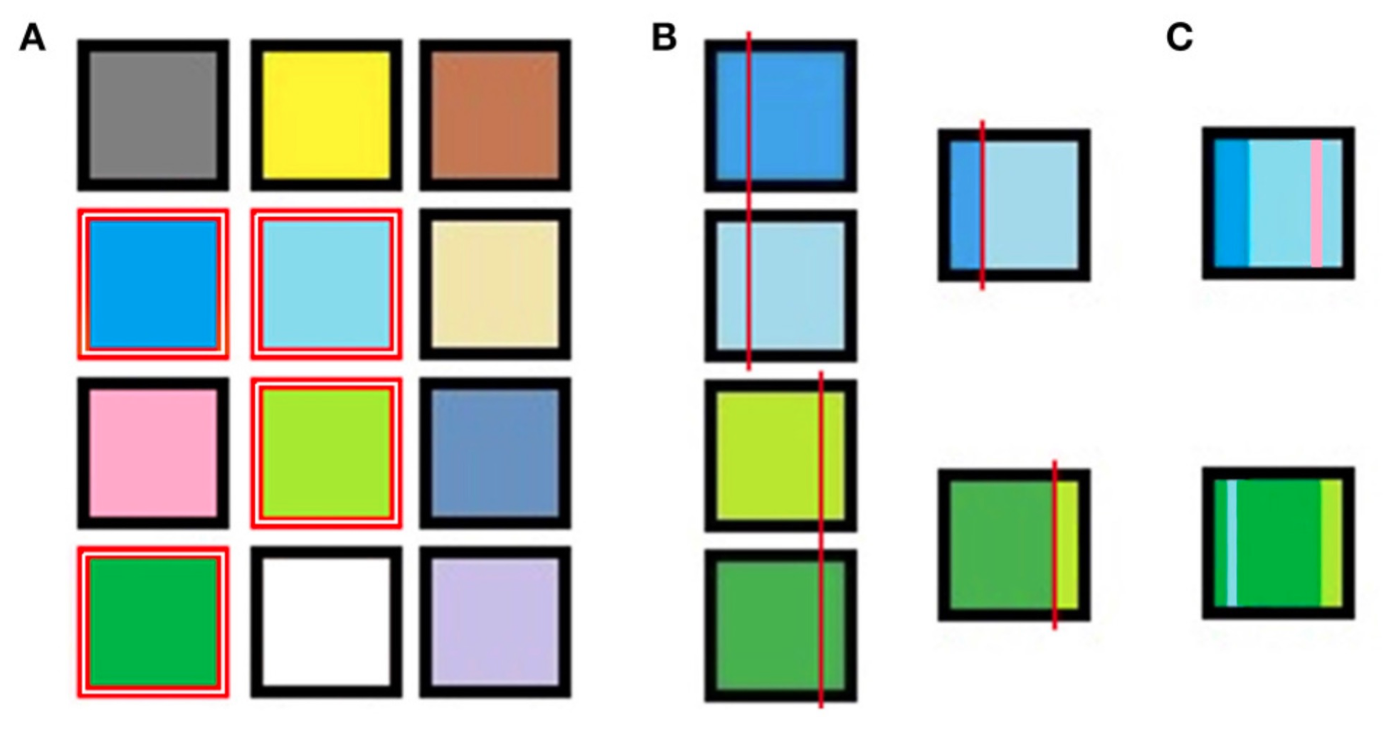
\includegraphics[width=0.5\textwidth]{ga_process.png}
\caption{From Reali et al 2017 - GA procedure example}
\end{figure}


\subsection{Genetic algorithm pseudocode}

\begin{figure}
\centering
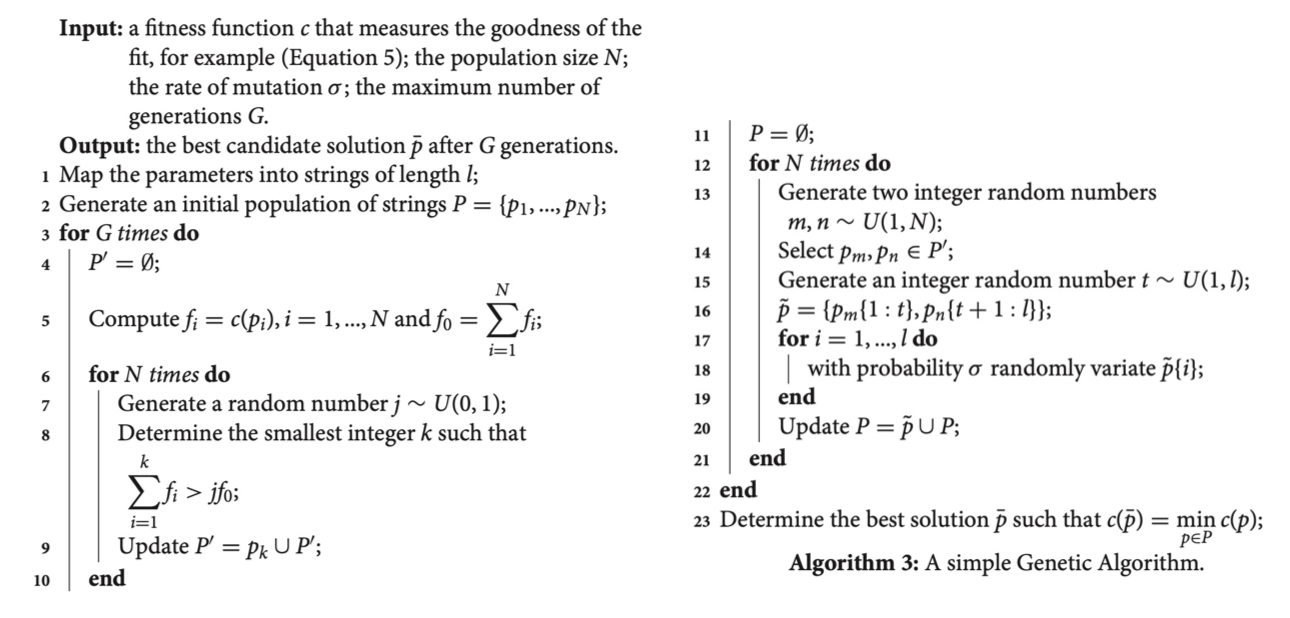
\includegraphics[width=0.8\textwidth]{ga_algo.png}
\caption{From Reali et al 2017 - GA pseudocode}
\end{figure}

\noindent
Observations on specifications:

\begin{enumerate}
\def\labelenumi{\arabic{enumi}.}
\tightlist
\item
  how many times do we go? Here we usually start by defining a number of
  generations
\item
  size of each population, use function to decide
\end{enumerate}

The cost function is as general as possible. GA is sometimes used for
hyperparameters tuning e.g.~we can train a NN inside the algorithm. This
is not feasible with Markov Chains or gradient methods.
\\
\\
\noindent
However, we do not know whether the new generation is better than the
previous one.

\subsubsection{Cons}

It is quite computationally demanding, as for N times we compute the
likelihood/cost/fitness just for selecting new parents. Next, we are not
directly getting direction, the reduction of the fitness function is not
driven by the dimension of the population. Close to the optimum it
converges slowly.

\subsubsection{Pros}

Each one of the computations can be parallelized. Some might argue that
it can be used for everything. It is very general and obtains good
results. \(f\) can vary sometimes; the algorithm can use an obj function
without the constraints, that can be added as penalties after some
generations.

